\documentclass[final]{fhnwreport}         %[mode] = draft or final

\let\counterwithout\relax
\let\counterwithin\relax
\usepackage{chngcntr}
%%---Main Packages-----------------------------------------------------------------------
\usepackage[english, ngerman]{babel}	%Mul­tilin­gual sup­port for LaTeX
\usepackage[OT1]{fontenc}				      %Stan­dard pack­age for se­lect­ing font en­cod­ings
\usepackage[utf8]{inputenc}				  %Ac­cept dif­fer­ent in­put en­cod­ings
%\usepackage{lmodern}                 %The newer Font-Set
%\usepackage{textcomp}					      %LaTeX sup­port for the Text Com­pan­ion fonts
\usepackage{graphicx} 					      %En­hanced sup­port for graph­ics
\usepackage{float}						        %Im­proved in­ter­face for float­ing ob­jects
%\usepackage{ifdraft}                %Let you check if the doc is in draft mode



%%---Useful Packages---------------------------------------------------------------------
%\usepackage[pdftex,dvipsnames,tables]{xcolor}  %Driver-in­de­pen­dent color ex­ten­sions for LaTeX
\usepackage{csquotes}                %Simpler quoting with \enquote{}
%\usepackage{siunitx} 					      %A com­pre­hen­sive (SI) units pack­age
\usepackage{listings}					      %Type­set source code list­ings us­ing LaTeX
%\usepackage[bottom]{footmisc}			  %A range of foot­note op­tions
\usepackage{footnote}					      %Im­prove on LaTeX's foot­note han­dling
%\usepackage{verbatim}					      %Reim­ple­men­ta­tion of and ex­ten­sions to LaTeX ver­ba­tim
%\usepackage[textsize=footnotesize]{todonotes} %Mark­ing things to do in a LaTeX doc­u­ment
\usepackage{lipsum}              % Gives you access to blindtext
\usepackage[most]{tcolorbox} % required by edit macros

% for dynamic spacing when defining using macros
\usepackage{xspace}
%emphasize still italic
\usepackage[normalem]{ulem} 
% enables itemize and enumerate within paragraphs (\begin{inparaenum}[i)])
\usepackage{paralist} 
% for icon next to scg URL next to author list on title page
\usepackage{fontawesome}   

%%---Tikz Packages-----------------------------------------------------------------------
%\usepackage{standalone}
%\usepackage{tikz}
%\usepackage{circuitikz}
%\usetikzlibrary{arrows}
%\usetikzlibrary{calc}
%\usetikzlibrary{intersections}

%%---Math Packages-----------------------------------------------------------------------
\usepackage{amsmath,amssymb,amsfonts, textcomp}					    %AMS math­e­mat­i­cal fa­cil­i­ties for LaTeX
%\usepackage{amssymb}					  %Type­set­ting symbols (AMS style)
%\usepackage{array}						  %Ex­tend­ing the ar­ray and tab­u­lar en­vi­ron­ments
%\usepackage{amsthm}					    %Type­set­ting the­o­rems (AMS style)

% boxes around text
\usepackage[framemethod=tikz]{mdframed}

% image alignment
\usepackage[export]{adjustbox}

% text alignment
\usepackage{ragged2e}

%%---Table Packages----------------------------------------------------------------------
%\usepackage{tabularx}					  %Tab­u­lars with ad­justable-width columns
\usepackage{multirow}					  %Create tab­u­lar cells span­ning mul­ti­ple rows
\usepackage{multicol}					  %In­ter­mix sin­gle and mul­ti­ple columns
\usepackage{longtable}
\usepackage{lscape}
\usepackage{array, booktabs} % improved table appearance and management (e.g., programmable column formats)
\usepackage{caption}
\usepackage{subcaption}

%%---PDF / Figure Packages---------------------------------------------------------------
\usepackage{pdfpages}					  %In­clude PDF doc­u­ments in LaTeX
\usepackage{pdflscape}					  %Make land­scape pages dis­play as land­scape
%\usepackage{subfig}					    %Fig­ures di­vided into sub­fig­ures

%%---Other Packages----------------------------------------------------------------------
%\usepackage{xargs}              %De­fine com­mands with many op­tional ar­gu­ments


%%---Main Settings-----------------------------------------------------------------------
\graphicspath{{./graphics/}}			%Defines the graphicspath
%\geometry{twoside=false}				%twoside=false disables the "bookstyle"
\setlength{\marginparwidth}{2cm}
\overfullrule=5em						    %Creates a black rule if text goes over the margins => debugging

%%---User Definitions--------------------------------------------------------------------
%%Tabel-Definitions: (requires \usepackage{tabularx})
\newcolumntype{L}[1]{>{\raggedright\arraybackslash}p{#1}}    %column-width and alignment
\newcolumntype{C}[1]{>{\centering\arraybackslash}p{#1}}
\newcolumntype{R}[1]{>{\raggedleft\arraybackslash}p{#1}}					                        %loads all packages, definitions and settings	
% Topic
\newcommand\topic[1]{\vspace{0.7em}
\noindent\textit{#1.}}


% ================================ %
% ======== BOXES AROUND TEXT ===== %
% ================================ %
\definecolor{mycolor}{rgb}{0.122, 0.435, 0.698}
\newmdenv[innerlinewidth=0.5pt, roundcorner=4pt,linecolor=mycolor,innerleftmargin=6pt,
innerrightmargin=6pt,innertopmargin=6pt,innerbottommargin=6pt]{mybox}
\newcommand{\finding}[1]{\begin{mybox}\emph{#1}\end{mybox}}




% Toggle: Put edit comments in a really ugly standout display, toggle to show or hide comments
\newboolean{showcomments}
\setboolean{showcomments}{true}
\ifthenelse{\boolean{showcomments}}
{\newcommand{\nbc}[3]{
{\colorbox{#3}{\bfseries\sffamily\scriptsize\textcolor{white}{#1}}}
{\textcolor{#3}{\sffamily\small$\blacktriangleright$\textit{#2}$\blacktriangleleft$}}}
\newcommand{\version}{\emph{\scriptsize\id}}}
{\newcommand{\nbc}[3]{}
\newcommand{\version}{}}

% Toggle: Mark-up macros for proof-reading, toggle to show or hide macros
\newboolean{showedits}
\setboolean{showedits}{true}
\ifthenelse{\boolean{showedits}}
{
\newcommand{\meh}[1]{\textcolor{red}{\uwave{#1}}} % please rephrase
\newcommand{\ins}[1]{\textcolor{blue}{\uline{#1}}} % please insert
\newcommand{\del}[1]{\textcolor{red}{\sout{#1}}} % please delete
\newcommand{\chg}[2]{\textcolor{red}{\sout{#1}}{\ra}\textcolor{blue}{\uline{#2}}} % please change
}{
\newcommand{\meh}[1]{#1} % please rephrase
\newcommand{\ins}[1]{#1} % please insert
\newcommand{\del}[1]{} % please delete
\newcommand{\chg}[2]{#2}
\newcommand{\nbe}[3]{}
}

% ===========================================

% Review macros (personalized)
\newcommand\on[1]{\nbc{ON}{#1}{olive}}
\newcommand\np[1]{\nbc{NP}{#1}{purple}}

% Review macros (generic)
\newcommand\fix[1]{\nbc{FIX}{#1}{orange}}
%\newcommand\todo[1]{\nbc{TO DO}{#1}{orange}}
\newcommand\msg[1]{\nbc{MESSAGE}{#1}{brown}}
\newcommand\fw[1]{\nbc{FUTUREWORK}{#1}{black}}
\newcommand\remind[1]{\nbc{REMINDER}{#1}{gray}}
\newcommand\review[1]{\nbc{TO REVIEW}{#1}{orange}}
\newcommand\ANS[1]{\nbe{Response}{#1}{teal}}
\newcommand\rA[1]{\nbe{Reviewer 1}{#1}{cyan}}
\newcommand\rB[1]{\nbe{Reviewer 2}{#1}{olive}}
\newcommand\rC[1]{\nbe{Reviewer 3}{#1}{magenta}}
\newcommand\rD[1]{\nbe{Reviewer 4}{#1}{orange}}

% Text shortcuts
\newcommand{\ie}{\emph{i.e.},\xspace}
\newcommand{\eg}{\emph{e.g.},\xspace}
\newcommand{\etal}{\emph{et al.}\xspace}
\newcommand{\etc}{\emph{etc.}\xspace}
\newcommand{\RQ}[1]{RQ$_{#1}$}

%%%%% Bibliographie entweder im IEEE- oder im APA-Stil:
\usepackage[style=ieee,urldate=comp,backend=biber]{biblatex}
%\usepackage[style=apa,urldate=comp,backend=biber]{biblatex}
%%%%%
\addbibresource{literature/beispiel_bib.bib}
											
\title{FHNW thesis template}  %Project Title
\author{Bachelor Thesis}    %Document Type => Technical Report, ...
\date{Windisch, August 20yy}               %Place and Date

\begin{document}

\pagenumbering{roman}	

%%---TITLEPAGE---------------------------------------------------------------------------
\selectlanguage{english}                  %ngerman or english
\maketitle

\vfill

\begin{figure}[H]
\centering
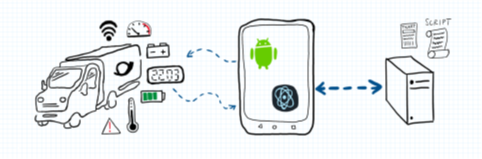
\includegraphics[width=\linewidth]{titleimage.png}
\end{figure}

\vfill

\begin{tabular}{@{}p{5cm} l}
Studentin/Student          &    Patrick Muster\\
                           &    Pia Mustermann\\[2ex]
Expertin/Experte           &    Gertrud Muster\\[2ex]
Fachbetreuer/in            &    Isidor Muster\\[2ex]
Auftraggeberin             &    Hans Muster, Mxxx\\[2ex]
Projektnummer              &    YXYX-S\\[4ex]
\multicolumn{2}{@{}l}{Fachhochschule Nordwestschweiz, Hochschule für Technik}
\end{tabular}

\vspace*{4ex}
% Beispiel für Logo Industriepartner
\begin{tikzpicture}[remember picture,overlay,every node/.style={anchor=north east}]
  \node at (current page.north east) [xshift=-1cm, yshift=-0.5cm] {
\includegraphics[width=4cm]{stoica-ionela-CoNsEK5iHug-unsplash.png}};
  % Photo by Stoica Ionela on Unsplash
\end{tikzpicture}
https://www.overleaf.com/project/624c2af918e86a2f5d4c45ec
\clearpage
			
%%---ABSTRACT----------------------------------------------------------------------------
\selectlanguage{english}				%ngerman or english
\thispagestyle{empty}
\section*{Abstract}
This is a sample text \np{let's try reviewing!}. 
\ins{Let's insert this}.
Patkar \etal
\del{Let's delete this}
%\chg{Let's change this}{ to that.}
This is a sample citation \cite{boser_hofmann_rezension_2015}.
\vspace{2ex}

\textbf{Keywords:}

tic, tac

\clearpage

\section*{Vorwort / Dank}




%%---TABLE OF CONTENTS-------------------------------------------------------------------	
\selectlanguage{english}				%ngerman or english
\tableofcontents
\clearpage

\listoffigures
\listoftables
\cleardoublepage

%%---TEXT--------------------------------------------------------------------------------
\pagenumbering{arabic}
\section{Introduction}

\section{State of the art}


\section{Sample chapter 1}

\subsection{Sample subsection}

\subsubsection{Sample subsubsection}

\section{Sample chapter 2}

\section{Conclusion and future work}




%%---BIBLIOGRAPHY------------------------------------------------------------------------
{\sloppypar
\printbibliography[heading=bibintoc, title=Quellenverzeichnis]
}

%%---APPENDIX----------------------------------------------------------------------------
\section*{Ehrlichkeitserklärung}
\addcontentsline{toc}{section}{Ehrlichkeitserklärung}

Hiermit erkläre ich, die vorliegende [Projektarbeit, Individualarbeit, Bachelorarbeit etc.] selbständig und nur unter Benutzung der angegebenen Quellen verfasst zu haben. Die wörtlich oder inhaltlich aus den aufgeführten Quellen entnommenen Stellen sind in der Arbeit als Zitat bzw. Paraphrase kenntlich gemacht. Diese [Studien-/Projektarbeit/Bachelor Thesis] ist noch nicht veröffentlicht worden. Sie ist somit weder anderen Interessierten zugänglich gemacht noch einer anderen Prüfungsbehörde vorgelegt worden.

\vspace*{4ex}

Windisch, tt. Monat 20jj

\vspace*{4ex}

{\renewcommand{\arraystretch}{2}
\begin{tabular}{@{}>{\bf}ll}
Name: & Pia Musterfrau\\
Unterschrift: & \\[6ex]
Name: & Michael Mustermann\\
Unterschrift: & \\
\end{tabular}
\begin{appendix} %Anhang
\section{Appendix 1}

\end{appendix}


%%---NOTES for DEBUG---------------------------------------------------------------------
%\newpage
%\listoftodos[\section{Todo-Notes}]
%\clearpage

\end{document}